\columnratio{0.55}
\begin{paracol}{2}
\switchcolumn[0]*%%%%%%%
\section{Template Syntax}
\switchcolumn
\section{模板语法}
\switchcolumn[0]*%%%%%%%
Vue uses an HTML-based template syntax that allows you to declaratively
bind the rendered DOM to the underlying component instance's data. All
Vue templates are syntactically valid HTML that can be parsed by
spec-compliant browsers and HTML parsers.
\switchcolumn
Vue 使用一种基于 HTML
的模板语法,使我们能够声明式地将其组件实例的数据绑定到呈现的 DOM
上。所有的 Vue 模板都是语法层面合法的 HTML,可以被符合规范的浏览器和
HTML 解析器解析。
\switchcolumn[0]*%%%%%%%
Under the hood, Vue compiles the templates into highly-optimized
JavaScript code. Combined with the reactivity system, Vue can
intelligently figure out the minimal number of components to re-render
and apply the minimal amount of DOM manipulations when the app state
changes.
\switchcolumn
在底层机制中,Vue 会将模板编译成高度优化的 JavaScript
代码。结合响应式系统,当应用状态变更时,Vue
能够智能地推导出需要重新渲染的组件的最少数量,并应用最少的 DOM 操作。
\switchcolumn[0]*%%%%%%%
If you are familiar with Virtual DOM concepts and prefer the raw power
of JavaScript, you can also
\href{https://vuejs.org/guide/extras/render-function.html}{directly
write render functions} instead of templates, with optional JSX support.
However, do note that they do not enjoy the same level of compile-time
optimizations as templates.
\switchcolumn
如果你对虚拟 DOM 的概念比较熟悉,并且偏好直接使用
JavaScript,你也可以结合可选的 JSX
支持\href{https://cn.vuejs.org/guide/extras/render-function.html}{直接手写渲染函数}而不采用模板。但请注意,这将不会享受到和模板同等级别的编译时优化。
\switchcolumn[0]*%%%%%%%
\subsection{Text Interpolation}
\switchcolumn
\subsection{文本插值}
\switchcolumn[0]*%%%%%%%
The most basic form of data binding is text interpolation using the
"Mustache" syntax (double curly braces):
\switchcolumn
最基本的数据绑定形式是文本插值,它使用的是``Mustache''语法
(即双大括号):
\switchcolumn[0]*%%%%%%%
\begin{codeHtml*}{label=template}
<span>Message: {{ msg }}</span>
\end{codeHtml*}  
\switchcolumn
\begin{codeHtml*}{label=template}
<span>Message: {{ msg }}</span>
\end{codeHtml*}  

\switchcolumn[0]*%%%%%%%
The mustache tag will be replaced with the value of the \texttt{msg}
property
\href{https://vuejs.org/guide/essentials/reactivity-fundamentals.html\#declaring-reactive-state}{from
the corresponding component instance}. It will also be updated whenever
the \texttt{msg} property changes.
\switchcolumn
双大括号标签会被替换为\href{https://cn.vuejs.org/guide/essentials/reactivity-fundamentals.html\#declaring-reactive-state}{相应组件实例中}
\texttt{msg} 属性的值。同时每次 \texttt{msg} 属性更改时它也会同步更新。
\switchcolumn[0]*%%%%%%%
\subsection{Raw HTML}
\switchcolumn
\subsection{原始 HTML}
\switchcolumn[0]*%%%%%%%
The double mustaches interpret the data as plain text, not HTML. In
order to output real HTML, you will need to use the
\href{https://vuejs.org/api/built-in-directives.html\#v-html}{\texttt{v-html}
directive}:
\switchcolumn
双大括号会将数据解释为纯文本,而不是 HTML。若想插入 HTML,你需要使用
\href{https://cn.vuejs.org/api/built-in-directives.html\#v-html}{\texttt{v-html}
指令}:
\switchcolumn[0]*%%%%%%%
\begin{codeHtml}
<p>Using text interpolation: {{ rawHtml }}</p>
<p>Using v-html directive: <span v-html="rawHtml"></span></p>
\end{codeHtml}  
\switchcolumn
\begin{codeHtml}
<p>Using text interpolation: {{ rawHtml }}</p>
<p>Using v-html directive: <span v-html="rawHtml"></span></p>
\end{codeHtml}  
\switchcolumn[0]*%%%%%%%
\begin{vueQuote}{result}
Using text interpolation: This should be red.\\
Using v-html directive: {\textcolor{red}{This should be red.}}
\end{vueQuote}
\switchcolumn
\begin{vueQuote}{结果}
Using text interpolation: This should be red.\\
Using v-html directive: {\textcolor{red}{This should be red.}}
\end{vueQuote}

\switchcolumn[0]*%%%%%%%
Here we're encountering something new. The \texttt{v-html} attribute
you're seeing is called a \textbf{directive}. Directives are prefixed
with \texttt{v-} to indicate that they are special attributes provided
by Vue, and as you may have guessed, they apply special reactive
behavior to the rendered DOM. Here, we're basically saying "keep this
element's inner HTML up-to-date with the \texttt{rawHtml} property on
the current active instance."
\switchcolumn
这里我们遇到了一个新的概念。这里看到的 \texttt{v-html} attribute
被称为一个\textbf{指令}。指令由 \texttt{v-} 作为前缀,表明它们是一些由
Vue 提供的特殊 attribute,你可能已经猜到了,它们将为渲染的 DOM
应用特殊的响应式行为。这里我们做的事情简单来说就是:在当前组件实例上,将此元素的
innerHTML 与 \texttt{rawHtml} 属性保持同步。
\switchcolumn[0]*%%%%%%%
The contents of the \texttt{span} will be replaced with the value of the
\texttt{rawHtml} property, interpreted as plain HTML - data bindings are
ignored. Note that you cannot use \texttt{v-html} to compose template
partials, because Vue is not a string-based templating engine. Instead,
components are preferred as the fundamental unit for UI reuse and
composition.
\switchcolumn
\texttt{span} 的内容将会被替换为 \texttt{rawHtml} 属性的值,插值为纯
HTML------数据绑定将会被忽略。注意,你不能使用 \texttt{v-html}
来拼接组合模板,因为 Vue 不是一个基于字符串的模板引擎。在使用 Vue
时,应当使用组件作为 UI 重用和组合的基本单元。
\switchcolumn[0]*%%%%%%%
\begin{vueQuoteWarn}{Security Warning}
Dynamically rendering arbitrary HTML on your website can be very
dangerous because it can easily lead to
\href{https://en.wikipedia.org/wiki/Cross-site_scripting}{XSS
vulnerabilities}. Only use \texttt{v-html} on trusted content and
\textbf{never} on user-provided content.
\end{vueQuoteWarn}
\switchcolumn
\begin{vueQuoteWarn}{安全警告}
在网站上动态渲染任意 HTML 是非常危险的,因为这非常容易造成
\href{https://zh.wikipedia.org/wiki/跨網站指令碼}{XSS
漏洞}。请仅在内容安全可信时再使用
\texttt{v-html},并且\textbf{永远不要}使用用户提供的 HTML 内容。
\end{vueQuoteWarn}
\switchcolumn[0]*%%%%%%%
\subsection{Attribute Bindings}
\switchcolumn
\subsection{Attribute 绑定}
\switchcolumn[0]*%%%%%%%
Mustaches cannot be used inside HTML attributes. Instead, use a
\href{https://vuejs.org/api/built-in-directives.html\#v-bind}{\texttt{v-bind}
directive}:
\switchcolumn
双大括号不能在 HTML attributes 中使用。想要响应式地绑定一个
attribute,应该使用
\href{https://cn.vuejs.org/api/built-in-directives.html\#v-bind}{\texttt{v-bind}
指令}:

\switchcolumn[0]*%%%%%%%
\begin{codeHtml}
<div v-bind:id="dynamicId"></div>
\end{codeHtml}  
\switchcolumn
\begin{codeHtml}
<div v-bind:id="dynamicId"></div>
\end{codeHtml}  
\switchcolumn[0]*%%%%%%%
The \texttt{v-bind} directive instructs Vue to keep the element's
\texttt{id} attribute in sync with the component's \texttt{dynamicId}
property. If the bound value is \texttt{null} or \texttt{undefined},
then the attribute will be removed from the rendered element.
\switchcolumn
\texttt{v-bind} 指令指示 Vue 将元素的 \texttt{id} attribute 与组件的
\texttt{dynamicId} 属性保持一致。如果绑定的值是 \texttt{null} 或者
\texttt{undefined},那么该 attribute 将会从渲染的元素上移除。
\switchcolumn[0]*%%%%%%%
\subsubsection{Shorthand}
\switchcolumn
\subsubsection{简写}
\switchcolumn[0]*%%%%%%%
Because \texttt{v-bind} is so commonly used, it has a dedicated
shorthand syntax:
\switchcolumn
因为 \texttt{v-bind} 非常常用,我们提供了特定的简写语法:


\switchcolumn[0]*%%%%%%%
\begin{codeHtml}
<div :id="dynamicId"></div>
\end{codeHtml}  
\switchcolumn
\begin{codeHtml}
<div :id="dynamicId"></div>
\end{codeHtml}  
\switchcolumn[0]*%%%%%%%
Attributes that start with \texttt{:} may look a bit different from
normal HTML, but it is in fact a valid character for attribute names and
all Vue-supported browsers can parse it correctly. In addition, they do
not appear in the final rendered markup. The shorthand syntax is
optional, but you will likely appreciate it when you learn more about
its usage later.
\switchcolumn
开头为 \texttt{:} 的 attribute 可能和一般的 HTML attribute
看起来不太一样,但它的确是合法的 attribute 名称字符,并且所有支持 Vue
的浏览器都能正确解析它。此外,他们不会出现在最终渲染的 DOM
中。简写语法是可选的,但相信在你了解了它更多的用处后,你应该会更喜欢它。
\switchcolumn[0]*%%%%%%%
\begin{quote}
For the rest of the guide, we will be using the shorthand syntax in code
examples, as that's the most common usage for Vue developers.
\end{quote}
\switchcolumn
\begin{quote}
接下来的指引中,我们都将在示例中使用简写语法,因为这是在实际开发中更常见的用法。
\end{quote}
\switchcolumn[0]*%%%%%%%
\subsubsection{Boolean Attributes}
\switchcolumn
\subsubsection{布尔型 Attribute}
\switchcolumn[0]*%%%%%%%
\href{https://html.spec.whatwg.org/multipage/common-microsyntaxes.html\#boolean-attributes}{Boolean
attributes} are attributes that can indicate true / false values by
their presence on an element. For example,
\href{https://developer.mozilla.org/en-US/docs/Web/HTML/Attributes/disabled}{\texttt{disabled}}
is one of the most commonly used boolean attributes.
\switchcolumn
\href{https://developer.mozilla.org/zh-CN/docs/Web/HTML/Attributes\#布尔值属性}{布尔型
attribute} 依据 true / false 值来决定 attribute
是否应该存在于该元素上。\href{https://developer.mozilla.org/en-US/docs/Web/HTML/Attributes/disabled}{\texttt{disabled}}
就是最常见的例子之一。
\switchcolumn[0]*%%%%%%%
\texttt{v-bind} works a bit differently in this case:
\switchcolumn
\texttt{v-bind} 在这种场景下的行为略有不同:

\switchcolumn[0]*%%%%%%%
\begin{codeHtml}
<button :disabled="isButtonDisabled">Button</button>
\end{codeHtml}  
\switchcolumn
\begin{codeHtml}
<button :disabled="isButtonDisabled">Button</button>
\end{codeHtml}  
\switchcolumn[0]*%%%%%%%
The \texttt{disabled} attribute will be included if
\texttt{isButtonDisabled} has a
\href{https://developer.mozilla.org/en-US/docs/Glossary/Truthy}{truthy
value}. It will also be included if the value is an empty string,
maintaining consistency with
\texttt{\textless{}button\ disabled=""\textgreater{}}. For other
\href{https://developer.mozilla.org/en-US/docs/Glossary/Falsy}{falsy
values} the attribute will be omitted.
\switchcolumn
当 \texttt{isButtonDisabled}
为\href{https://developer.mozilla.org/en-US/docs/Glossary/Truthy}{真值}或一个空字符串
(即 \texttt{\textless{}button\ disabled=""\textgreater{}})
时,元素会包含这个 \texttt{disabled}
attribute。而当其为其他\href{https://developer.mozilla.org/en-US/docs/Glossary/Falsy}{假值}时
attribute 将被忽略。
\switchcolumn[0]*%%%%%%%
\subsubsection{Dynamically Binding Multiple Attributes}
\switchcolumn
\subsubsection{动态绑定多个值}
\switchcolumn[0]*%%%%%%%
If you have a JavaScript object representing multiple attributes that
looks like this:
\switchcolumn
如果你有像这样的一个包含多个 attribute 的 JavaScript 对象:
\switchcolumn[0]*%%%%%%%
\begin{codeJs}
const objectOfAttrs = {
  id: 'container',
  class: 'wrapper'
}
\end{codeJs}
\switchcolumn
\begin{codeJs}
const objectOfAttrs = {
  id: 'container',
  class: 'wrapper'
}
\end{codeJs}
\switchcolumn[0]*%%%%%%%
You can bind them to a single element by using \texttt{v-bind} without
an argument:
\switchcolumn
通过不带参数的 \texttt{v-bind},你可以将它们绑定到单个元素上:
\switchcolumn[0]*%%%%%%%
\begin{codeHtml}
<div v-bind="objectOfAttrs"></div>
\end{codeHtml}  
\switchcolumn
\begin{codeHtml}
<div v-bind="objectOfAttrs"></div>
\end{codeHtml}  
\switchcolumn[0]*%%%%%%%
\subsection{Using JavaScript Expressions}
\switchcolumn
\subsection{使用 JavaScript 表达式}
\switchcolumn[0]*%%%%%%%
So far we've only been binding to simple property keys in our templates.
But Vue actually supports the full power of JavaScript expressions
inside all data bindings:
\switchcolumn
至此,我们仅在模板中绑定了一些简单的属性名。但是 Vue
实际上在所有的数据绑定中都支持完整的 JavaScript 表达式:

\switchcolumn[0]*%%%%%%%
\begin{codeHtml}
{{ number + 1 }}

{{ ok ? 'YES' : 'NO' }}

{{ message.split('').reverse().join('') }}

<div :id="`list-${id}`"></div>
\end{codeHtml}
\switchcolumn
\begin{codeHtml}
{{ number + 1 }}

{{ ok ? 'YES' : 'NO' }}

{{ message.split('').reverse().join('') }}

<div :id="`list-${id}`"></div>
\end{codeHtml}

\switchcolumn[0]*%%%%%%%
These expressions will be evaluated as JavaScript in the data scope of
the current component instance.
\switchcolumn
这些表达式都会被作为 JavaScript ,以当前组件实例为作用域解析执行。
\switchcolumn[0]*%%%%%%%
In Vue templates, JavaScript expressions can be used in the following
positions:
\switchcolumn
在 Vue 模板内,JavaScript 表达式可以被使用在如下场景上:

\switchcolumn[0]*%%%%%%%
\begin{itemize}
\item
Inside text interpolations (mustaches)
\item
In the attribute value of any Vue directives (special attributes that
start with \texttt{v-})
\end{itemize}
\switchcolumn
\begin{itemize}
\item
在文本插值中 (双大括号)
\item
在任何 Vue 指令 (以 \texttt{v-} 开头的特殊 attribute) attribute 的值中
\end{itemize}

\switchcolumn[0]*%%%%%%%
\subsubsection{Expressions Only}
\switchcolumn
\subsubsection{仅支持表达式}
\switchcolumn[0]*%%%%%%%
Each binding can only contain \textbf{one single expression}. An
expression is a piece of code that can be evaluated to a value. A simple
check is whether it can be used after \texttt{return}.
\switchcolumn
每个绑定仅支持\textbf{单一表达式},也就是一段能够被求值的 JavaScript
代码。一个简单的判断方法是是否可以合法地写在 \texttt{return} 后面。
\switchcolumn[0]*%%%%%%%
Therefore, the following will \textbf{NOT} work:
\switchcolumn
因此,下面的例子都是\textbf{无效}的:
\switchcolumn[0]*%%%%%%%
\begin{codeHtml}
<!-- this is a statement, not an expression: -->
{{ var a = 1 }}

<!-- flow control won't work either, use ternary expressions -->
{{ if (ok) { return message } }}
\end{codeHtml}  
\switchcolumn
\begin{codeHtml}
<!-- 这是一个语句,而非表达式 -->
{{ var a = 1 }}

<!-- 条件控制也不支持,请使用三元表达式 -->
{{ if (ok) { return message } }}
\end{codeHtml}  

\switchcolumn[0]*%%%%%%%
\subsubsection{Calling Functions}
\switchcolumn
\subsubsection{调用函数}
\switchcolumn[0]*%%%%%%%
It is possible to call a component-exposed method inside a binding
expression:
\switchcolumn
可以在绑定的表达式中使用一个组件暴露的方法:
\switchcolumn[0]*%%%%%%%
\begin{codeHtml}
<time :title="toTitleDate(date)" :datetime="date">
{{ formatDate(date) }}
</time>
\end{codeHtml}  
\switchcolumn
\begin{codeHtml}
<time :title="toTitleDate(date)" :datetime="date">
{{ formatDate(date) }}
</time>
\end{codeHtml}  
\switchcolumn[0]*%%%%%%%
\begin{vueQuote}{TIP}
Functions called inside binding expressions will be called every time
the component updates, so they should \textbf{not} have any side
effects, such as changing data or triggering asynchronous operations.
\end{vueQuote}
\switchcolumn
\begin{vueQuote}{TIP}
绑定在表达式中的方法在组件每次更新时都会被重新调用,因此\textbf{不}应该产生任何副作用,比如改变数据或触发异步操作。
\end{vueQuote}

\switchcolumn[0]*%%%%%%%
\subsubsection{Restricted Globals Access}
\switchcolumn
\subsubsection{受限的全局访问}
\switchcolumn[0]*%%%%%%%
Template expressions are sandboxed and only have access to a
\href{https://github.com/vuejs/core/blob/main/packages/shared/src/globalsAllowList.ts\#L3}{restricted
list of globals}. The list exposes commonly used built-in globals such
as \texttt{Math} and \texttt{Date}.
\switchcolumn
模板中的表达式将被沙盒化,仅能够访问到\href{https://github.com/vuejs/core/blob/main/packages/shared/src/globalsAllowList.ts\#L3}{有限的全局对象列表}。该列表中会暴露常用的内置全局对象,比如
\texttt{Math} 和 \texttt{Date}。
\switchcolumn[0]*%%%%%%%
Globals not explicitly included in the list, for example user-attached
properties on \texttt{window}, will not be accessible in template
expressions. You can, however, explicitly define additional globals for
all Vue expressions by adding them to
\href{https://vuejs.org/api/application.html\#app-config-globalproperties}{\texttt{app.config.globalProperties}}.
\switchcolumn
没有显式包含在列表中的全局对象将不能在模板内表达式中访问,例如用户附加在
\texttt{window} 上的属性。然而,你也可以自行在
\href{https://cn.vuejs.org/api/application.html\#app-config-globalproperties}{\texttt{app.config.globalProperties}}
上显式地添加它们,供所有的 Vue 表达式使用。
\switchcolumn[0]*%%%%%%%
\subsection{Directives}
\switchcolumn
\subsection{指令 Directives}
\switchcolumn[0]*%%%%%%%
Directives are special attributes with the \texttt{v-} prefix. Vue
provides a number of
\href{https://vuejs.org/api/built-in-directives.html}{built-in
directives}, including \texttt{v-html} and \texttt{v-bind} which we have
introduced above.
\switchcolumn
指令是带有 \texttt{v-} 前缀的特殊 attribute。Vue
提供了许多\href{https://cn.vuejs.org/api/built-in-directives.html}{内置指令},包括上面我们所介绍的
\texttt{v-bind} 和 \texttt{v-html}。
\switchcolumn[0]*%%%%%%%
Directive attribute values are expected to be single JavaScript
expressions (with the exception of \texttt{v-for}, \texttt{v-on} and
\texttt{v-slot}, which will be discussed in their respective sections
later). A directive's job is to reactively apply updates to the DOM when
the value of its expression changes. Take
\href{https://vuejs.org/api/built-in-directives.html\#v-if}{\texttt{v-if}}
as an example:
\switchcolumn
指令 attribute 的期望值为一个 JavaScript 表达式
(除了少数几个例外,即之后要讨论到的 \texttt{v-for}、\texttt{v-on} 和
\texttt{v-slot})。一个指令的任务是在其表达式的值变化时响应式地更新
DOM。以
\href{https://cn.vuejs.org/api/built-in-directives.html\#v-if}{\texttt{v-if}}
为例:

\switchcolumn[0]*%%%%%%%
\begin{codeHtml}
<p v-if="seen">Now you see me</p>
\end{codeHtml}  
\switchcolumn
\begin{codeHtml}
<p v-if="seen">Now you see me</p>
\end{codeHtml}  
\switchcolumn[0]*%%%%%%%
Here, the \texttt{v-if} directive would remove / insert the
\texttt{\textless{}p\textgreater{}} element based on the truthiness of
the value of the expression \texttt{seen}.
\switchcolumn
这里,\texttt{v-if} 指令会基于表达式 \texttt{seen}
的值的真假来移除/插入该 \texttt{\textless{}p\textgreater{}} 元素。
\switchcolumn[0]*%%%%%%%
\subsubsection{Arguments}
\switchcolumn
\subsubsection{参数 Arguments}
\switchcolumn[0]*%%%%%%%
Some directives can take an "argument", denoted by a colon after the
directive name. For example, the \texttt{v-bind} directive is used to
reactively update an HTML attribute:
\switchcolumn
某些指令会需要一个``参数'',在指令名后通过一个冒号隔开做标识。例如用
\texttt{v-bind} 指令来响应式地更新一个 HTML attribute:

\switchcolumn[0]*%%%%%%%
\begin{codeHtml}
<a v-bind:href="url"> ... </a>

<!-- shorthand -->
<a :href="url"> ... </a>
\end{codeHtml}  
\switchcolumn
\begin{codeHtml}
<a v-bind:href="url"> ... </a>

<!-- 简写 -->
<a :href="url"> ... </a>
\end{codeHtml}  

\switchcolumn[0]*%%%%%%%
Here, \texttt{href} is the argument, which tells the \texttt{v-bind}
directive to bind the element's \texttt{href} attribute to the value of
the expression \texttt{url}. In the shorthand, everything before the
argument (i.e., \texttt{v-bind:}) is condensed into a single character,
\texttt{:}.
\switchcolumn
这里 \texttt{href} 就是一个参数,它告诉 \texttt{v-bind} 指令将表达式
\texttt{url} 的值绑定到元素的 \texttt{href} attribute
上。在简写中,参数前的一切 (例如 \texttt{v-bind:}) 都会被缩略为一个
\texttt{:} 字符。
\switchcolumn[0]*%%%%%%%
Another example is the \texttt{v-on} directive, which listens to DOM
events:
\switchcolumn
另一个例子是 \texttt{v-on} 指令,它将监听 DOM 事件:
\switchcolumn[0]*%%%%%%%
\begin{codeHtml}
<a v-on:click="doSomething"> ... </a>

<!-- shorthand -->
<a @click="doSomething"> ... </a>
\end{codeHtml}  
\switchcolumn
\begin{codeHtml}
<a v-on:click="doSomething"> ... </a>

<!-- 简写 -->
<a @click="doSomething"> ... </a>
\end{codeHtml}  

\switchcolumn[0]*%%%%%%%
Here, the argument is the event name to listen to: \texttt{click}.
\texttt{v-on} has a corresponding shorthand, namely the \texttt{@}
character. We will talk about event handling in more detail too.
\switchcolumn
这里的参数是要监听的事件名称:\texttt{click}。\texttt{v-on}
有一个相应的缩写,即 \texttt{@}
字符。我们之后也会讨论关于事件处理的更多细节。
\switchcolumn[0]*%%%%%%%
\subsubsection{Dynamic Arguments}
\switchcolumn
\subsubsection{动态参数}
\switchcolumn[0]*%%%%%%%
It is also possible to use a JavaScript expression in a directive
argument by wrapping it with square brackets:
\switchcolumn
同样在指令参数上也可以使用一个 JavaScript
表达式,需要包含在一对方括号内:
\switchcolumn[0]*%%%%%%%
\begin{codeHtml}
<!--
Note that there are some constraints to the argument expression,
as explained in the "Dynamic Argument Value Constraints" 
and "Dynamic Argument Syntax Constraints" sections below.
-->
<a v-bind:[attributeName]="url"> ... </a>

<!-- shorthand -->
<a :[attributeName]="url"> ... </a>
\end{codeHtml}  
\switchcolumn
\begin{codeHtml}
<!--
注意,参数表达式有一些约束,
参见下面“动态参数值的限制”与“动态参数语法的限制”章节的解释
-->
<a v-bind:[attributeName]="url"> ... </a>

<!-- 简写 -->
<a :[attributeName]="url"> ... </a>
\end{codeHtml}  

\switchcolumn[0]*%%%%%%%
Here, \texttt{attributeName} will be dynamically evaluated as a
JavaScript expression, and its evaluated value will be used as the final
value for the argument. For example, if your component instance has a
data property, \texttt{attributeName}, whose value is \texttt{"href"},
then this binding will be equivalent to \texttt{v-bind:href}.
\switchcolumn
这里的 \texttt{attributeName} 会作为一个 JavaScript
表达式被动态执行,计算得到的值会被用作最终的参数。举例来说,如果你的组件实例有一个数据属性
\texttt{attributeName},其值为 \texttt{"href"},那么这个绑定就等价于
\texttt{v-bind:href}。
\switchcolumn[0]*%%%%%%%
Similarly, you can use dynamic arguments to bind a handler to a dynamic
event name:
\switchcolumn
相似地,你还可以将一个函数绑定到动态的事件名称上:
\switchcolumn[0]*%%%%%%%
\begin{codeHtml}
<a v-on:[eventName]="doSomething"> ... </a>

<!-- shorthand -->
<a @[eventName]="doSomething">
\end{codeHtml}  
\switchcolumn
\begin{codeHtml}
<a v-on:[eventName]="doSomething"> ... </a>

<!-- 简写 -->
<a @[eventName]="doSomething">
\end{codeHtml}  
\switchcolumn[0]*%%%%%%%
In this example, when \texttt{eventName}'s value is \texttt{"focus"},
\texttt{v-on:{[}eventName{]}} will be equivalent to \texttt{v-on:focus}.
\switchcolumn
在此示例中,当 \texttt{eventName} 的值是 \texttt{"focus"}
时,\texttt{v-on:{[}eventName{]}} 就等价于 \texttt{v-on:focus}。 
\switchcolumn[0]*%%%%%%% 
\subsubsection{Dynamic Argument Value Constraints}%%%%%%todo bug v如果单个paragraph放一个栏环境,中文会替代英文

Dynamic arguments are expected to evaluate to a string, with the
exception of \texttt{null}. The special value \texttt{null} can be used
to explicitly remove the binding. Any other non-string value will
trigger a warning.
\switchcolumn
\subsubsection{动态参数值的限制}

动态参数中表达式的值应当是一个字符串,或者是 \texttt{null}。特殊值
\texttt{null} 意为显式移除该绑定。其他非字符串的值会触发警告。

\switchcolumn[0]*%%%%%%%
\subsubsection{Dynamic Argument Syntax Constraints}

Dynamic argument expressions have some syntax constraints because
certain characters, such as spaces and quotes, are invalid inside HTML
attribute names. For example, the following is invalid:
\switchcolumn
\subsubsection{动态参数语法的限制}

动态参数表达式因为某些字符的缘故有一些语法限制,比如空格和引号,在 HTML
attribute 名称中都是不合法的。例如下面的示例:

\switchcolumn[0]*%%%%%%%
\begin{codeHtml}
<!-- This will trigger a compiler warning. -->
<a :['foo' + bar]="value"> ... </a>
\end{codeHtml}  
\switchcolumn
\begin{codeHtml} 
<!-- 这会触发一个编译器警告 -->
<a :['foo' + bar]="value"> ... </a>
\end{codeHtml}  
\switchcolumn[0]*%%%%%%%
If you need to pass a complex dynamic argument, it's probably better to
use a \href{https://vuejs.org/guide/essentials/computed.html}{computed
property}, which we will cover shortly.
\switchcolumn
如果你需要传入一个复杂的动态参数,我们推荐使用\href{https://cn.vuejs.org/guide/essentials/computed.html}{计算属性}替换复杂的表达式,也是
Vue 最基础的概念之一,我们很快就会讲到。
\switchcolumn[0]*%%%%%%%
When using in-DOM templates (templates directly written in an HTML
file), you should also avoid naming keys with uppercase characters, as
browsers will coerce attribute names into lowercase:
\switchcolumn
当使用 DOM 内嵌模板 (直接写在 HTML 文件里的模板)
时,我们需要避免在名称中使用大写字母,因为浏览器会强制将其转换为小写:
\switchcolumn[0]*%%%%%%%
\begin{codeHtml}
<a :[someAttr]="value"> ... </a>
\end{codeHtml}  
\switchcolumn
\begin{codeHtml}
<a :[someAttr]="value"> ... </a>
\end{codeHtml}  
\switchcolumn[0]*%%%%%%%
The above will be converted to \texttt{:{[}someattr{]}} in in-DOM
templates. If your component has a \texttt{someAttr} property instead of
\texttt{someattr}, your code won't work. Templates inside Single-File
Components are \textbf{not} subject to this constraint.
\switchcolumn
上面的例子将会在 DOM 内嵌模板中被转换为
\texttt{:{[}someattr{]}}。如果你的组件拥有 ``someAttr'' 属性而非
``someattr'',这段代码将不会工作。单文件组件内的模板\textbf{不}受此限制。
\switchcolumn[0]*%%%%%%%
\subsubsection{Modifiers}
\switchcolumn
\subsubsection{修饰符 Modifiers}
\switchcolumn[0]*%%%%%%%
Modifiers are special postfixes denoted by a dot, which indicate that a
directive should be bound in some special way. For example, the
\texttt{.prevent} modifier tells the \texttt{v-on} directive to call
\\\texttt{event.preventDefault()} on the triggered event:
\switchcolumn
修饰符是以点开头的特殊后缀,表明指令需要以一些特殊的方式被绑定。例如
\texttt{.prevent} 修饰符会告知 \texttt{v-on} 指令对触发的事件调用
\texttt{event.preventDefault()}:
\switchcolumn[0]*%%%%%%%
\begin{codeHtml}
<form @submit.prevent="onSubmit">...</form>
\end{codeHtml}  
\switchcolumn
\begin{codeHtml}
<form @submit.prevent="onSubmit">...</form>
\end{codeHtml}  
\switchcolumn[0]*%%%%%%%
You'll see other examples of modifiers later,
\href{https://vuejs.org/guide/essentials/event-handling.html\#event-modifiers}{for
\texttt{v-on}} and
\href{https://vuejs.org/guide/essentials/forms.html\#modifiers}{for
\texttt{v-model}}, when we explore those features.
\switchcolumn
之后在讲到
\href{https://cn.vuejs.org/guide/essentials/event-handling.html\#event-modifiers}{\texttt{v-on}}
和
\href{https://cn.vuejs.org/guide/essentials/forms.html\#modifiers}{\texttt{v-model}}
的功能时,你将会看到其他修饰符的例子。
\switchcolumn[0]*%%%%%%%
And finally, here's the full directive syntax visualized:
\switchcolumn
最后,在这里你可以直观地看到完整的指令语法:
\end{paracol}
\begin{center} 
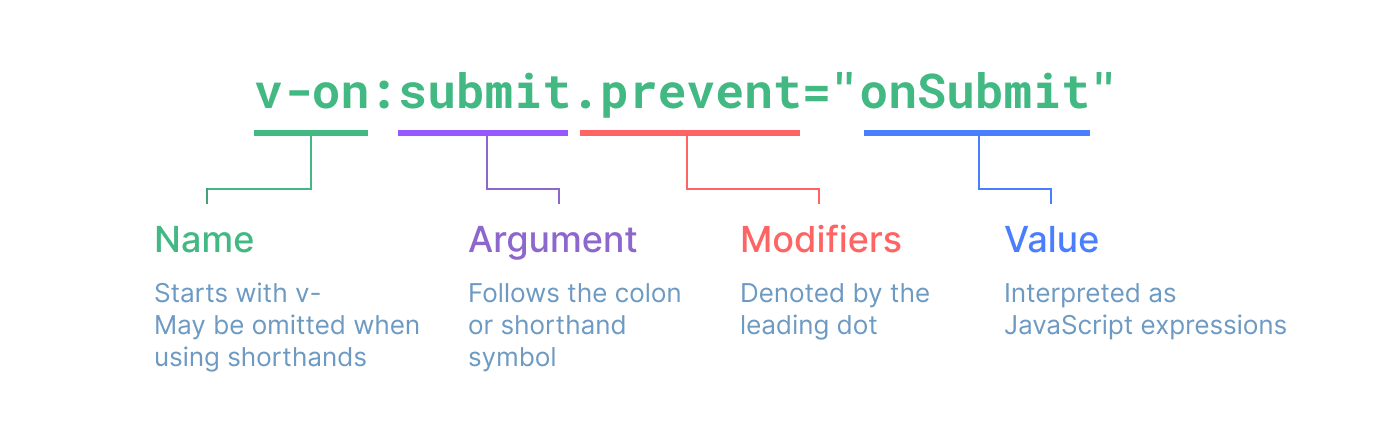
\includegraphics{./img/directive.69c37117.png} 
\end{center}
